\documentclass{beamer}
\usepackage{subcaption} 
\title{Using AMPL inside C}
\author{Johnathan Rhyne}
\institute{CU Denver}
\date{\today}
\usetheme{Rochester}
\begin{document}
    \frame{\titlepage}
    \begin{frame}
        \frametitle{Table of Contents}
        \tableofcontents
    \end{frame}
    \section{Brief AMPL Overview}
    \begin{frame}
        \frametitle{What is AMPL?}
        AMPL Stands for \textbf{A} \textbf{M}athematical \textbf{P}rogramming \textbf{L}anguage.

        In short, it is a relatively
        human readable way of asking a computer to solve optimization problems for us.
    \end{frame}
    \section{Problem Overview}
    \begin{frame}
        \frametitle{What is Sudoku?}
        \begin{figure}
            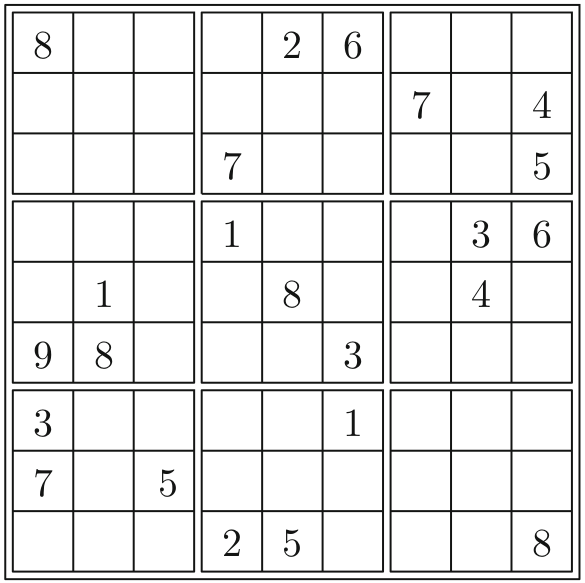
\includegraphics[scale=0.25]{figures/sudokuGrid.png}
            \caption{Source: Integer Programming - Michele conforti Gerard Cornuejols Giacomo Zambelli}
        \end{figure}
    \end{frame}
    \begin{frame}
        \frametitle{Sudoku as an Integer Program}
        \footnotesize
        \begin{align*}
            \sum_{i=1}^9 x_{ijk} = 1&,\qquad 1\leq jk\leq 9\qquad\qquad\text{(each number $k$ appears in each column)}\\
            \sum_{j=1}^9 x_{ijk} = 1&,\qquad 1\leq ik\leq 9\qquad\qquad\text{(each number $k$ appears in each row)} \\
            \sum_{q,r=0}^2x_{i+q,j+r,k} = 1&, \qquad i,j=1,4,7,\, 1\leq k \leq 9 \qquad\text{(each $k$ appears once in each box)}\\
            \sum_{k=1}^9 x_{ijk} = 1&,\qquad 1\leq ij\leq 9\qquad\qquad\text{(each cell contains exactly one number)} \\
            x_{ijk}\in\{0,1\} &, \qquad 1\leq ijk\leq 9 \\
            x_{ijk} = 1 &,  \qquad\text{When the initial board has number $k$ in cell $(i,j)$.}
        \end{align*}
    \end{frame}
    \section{Embedding in C}
    \subsection{Files Created Externally}
    \begin{frame}
        \frametitle{Use Case For External File Creation}
        \begin{itemize}
            \item Already tried running it locally, so you have the files
            \item Running on a cluster with no GUI or very high latency
            \item Only part of what you are trying to solve
        \end{itemize}
    \end{frame}
    \begin{frame}
        \frametitle{Requirements}
        \begin{itemize}
            \item AMPL installation accessible to your user
            \item A list of AMPL commands inside a text file
        \end{itemize}
    \end{frame}
    \begin{frame}
        \frametitle{Example AMPL Files}
        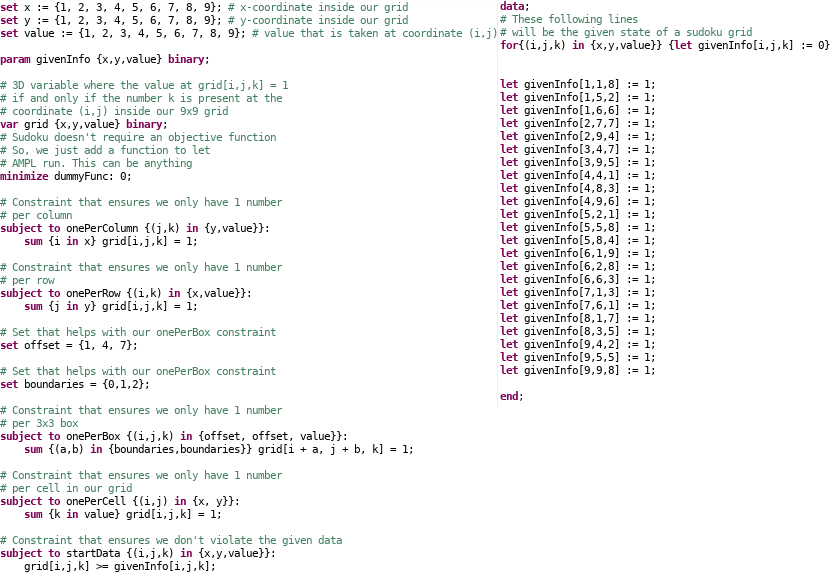
\includegraphics[width=\textwidth]{figures/presentationFile.png}
   \end{frame}
   \begin{frame}
        \frametitle{Command File}
        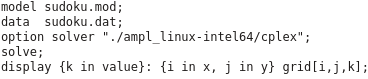
\includegraphics[width=\textwidth]{figures/sudokuCommand.png}
   \end{frame}
   \begin{frame}
       \frametitle{Calling From C!}
        system(amplPath \textless \, commandFilePath \textgreater \,outputFilePath)
   \end{frame}
   \begin{frame}
       \frametitle{Nice Output}
        \centering
        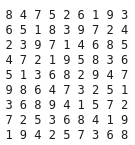
\includegraphics[scale=.75]{figures/exampleOutput.png}
   \end{frame}
    \subsection{All Inside C}
    \begin{frame}
        \frametitle{All Inside C: Key Things to Consider}
        \begin{itemize}
            \item No official API like Java, Python, C++
            \item However, can do most of it through basic File I/O and system calls!
        \end{itemize}
    \end{frame}
    \begin{frame}
        \frametitle{Example C File}
        \centering
        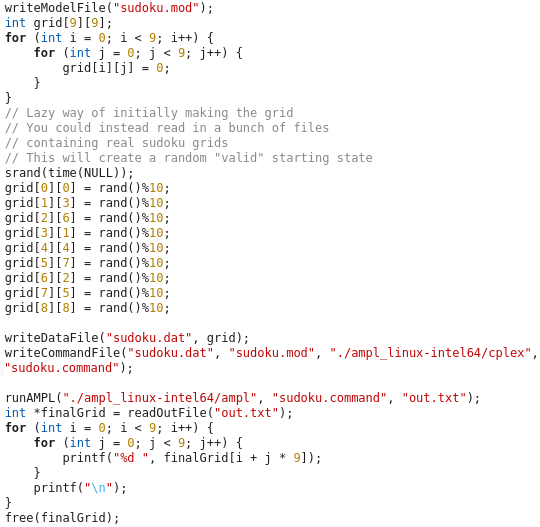
\includegraphics[scale=.35]{figures/insideCCode.png}
    \end{frame}
    \begin{frame}
        \frametitle{Example Output}
        \centering
        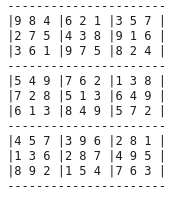
\includegraphics[scale=.75]{figures/randomOutput.png}
    \end{frame}
    \section{Extensions}
    \begin{frame}
        \frametitle{Variant Sudoku}
        \begin{itemize}
            \item Arrow Sum Lines
            \item Killer Boxes
        \end{itemize}
    \end{frame}
\end{document}
